\documentclass[conference]{IEEEtran} % Usa la classe IEEEtran per formattazione simile

\usepackage{amsmath}
\usepackage{graphicx}



\begin{document}

\title{Exploring the Adversarial Robustness of AI-generated Image Detectors}

\author{
    \IEEEauthorblockN{Thomas Lazzerini, Samuele Cappelletti, Martina D'Angelo}
    \IEEEauthorblockA{
        University of Trento
    }
}

\maketitle

\begin{abstract}
    %METTIAMO????
\end{abstract}

\section{Introduction}
    Synthetic images are now flooding the real world. From online dating sites to social media, fake profiles and scams are everywhere. The problem with synthetic images is that, while some of them are funny and harmless, others could be harmful, they could be exploited by malicious users. In relation to this, in the image forensic field there is a continuous fight between \textit{fake image detectors} and \textit{adversarial attacks}. On one hand, the detectors try to distinguish fake images from real ones, while, on the other hand, the attacks try to trick the detectors by manipulating the images (both real and fake ones). In order to detect fake images, we can exploit the traces/artifacts that fake image generators leave on the generated images. To do so, we have two main types of techniques: the \textit{low-level forensic techniques} and the \textit{high-level forensic techniques}. To former focuses on the pixel-level artifacts, which are almost invisible to the human eye. The latter focuses on physical inconsistencies and on repeated and uniform patterns, both of which are mostly visible to the human eye. Examples of physical inconsistencies are lighting, shadows, reflections or vanishing points inconsistencies. While, an example of repeated and uniform patterns, typical of GAN-based image generators, is the generation of the mouth, the nose and the eyes always in the same position. In general, we prefer to rely on low-level artifacts since fake image generators are becoming smarter every day, thus they are learning to generate always more realistic images, with fewer physical inconsistencies.


    METTERE LE REFERENCE IN INTRODUCTION


    \cite{zhu2005semi}
    %As discussed in \cite{zhu2005semi}, semi-supervised learning is an important area of research.

    %\begin{figure}[h]
    %    \centering
    %    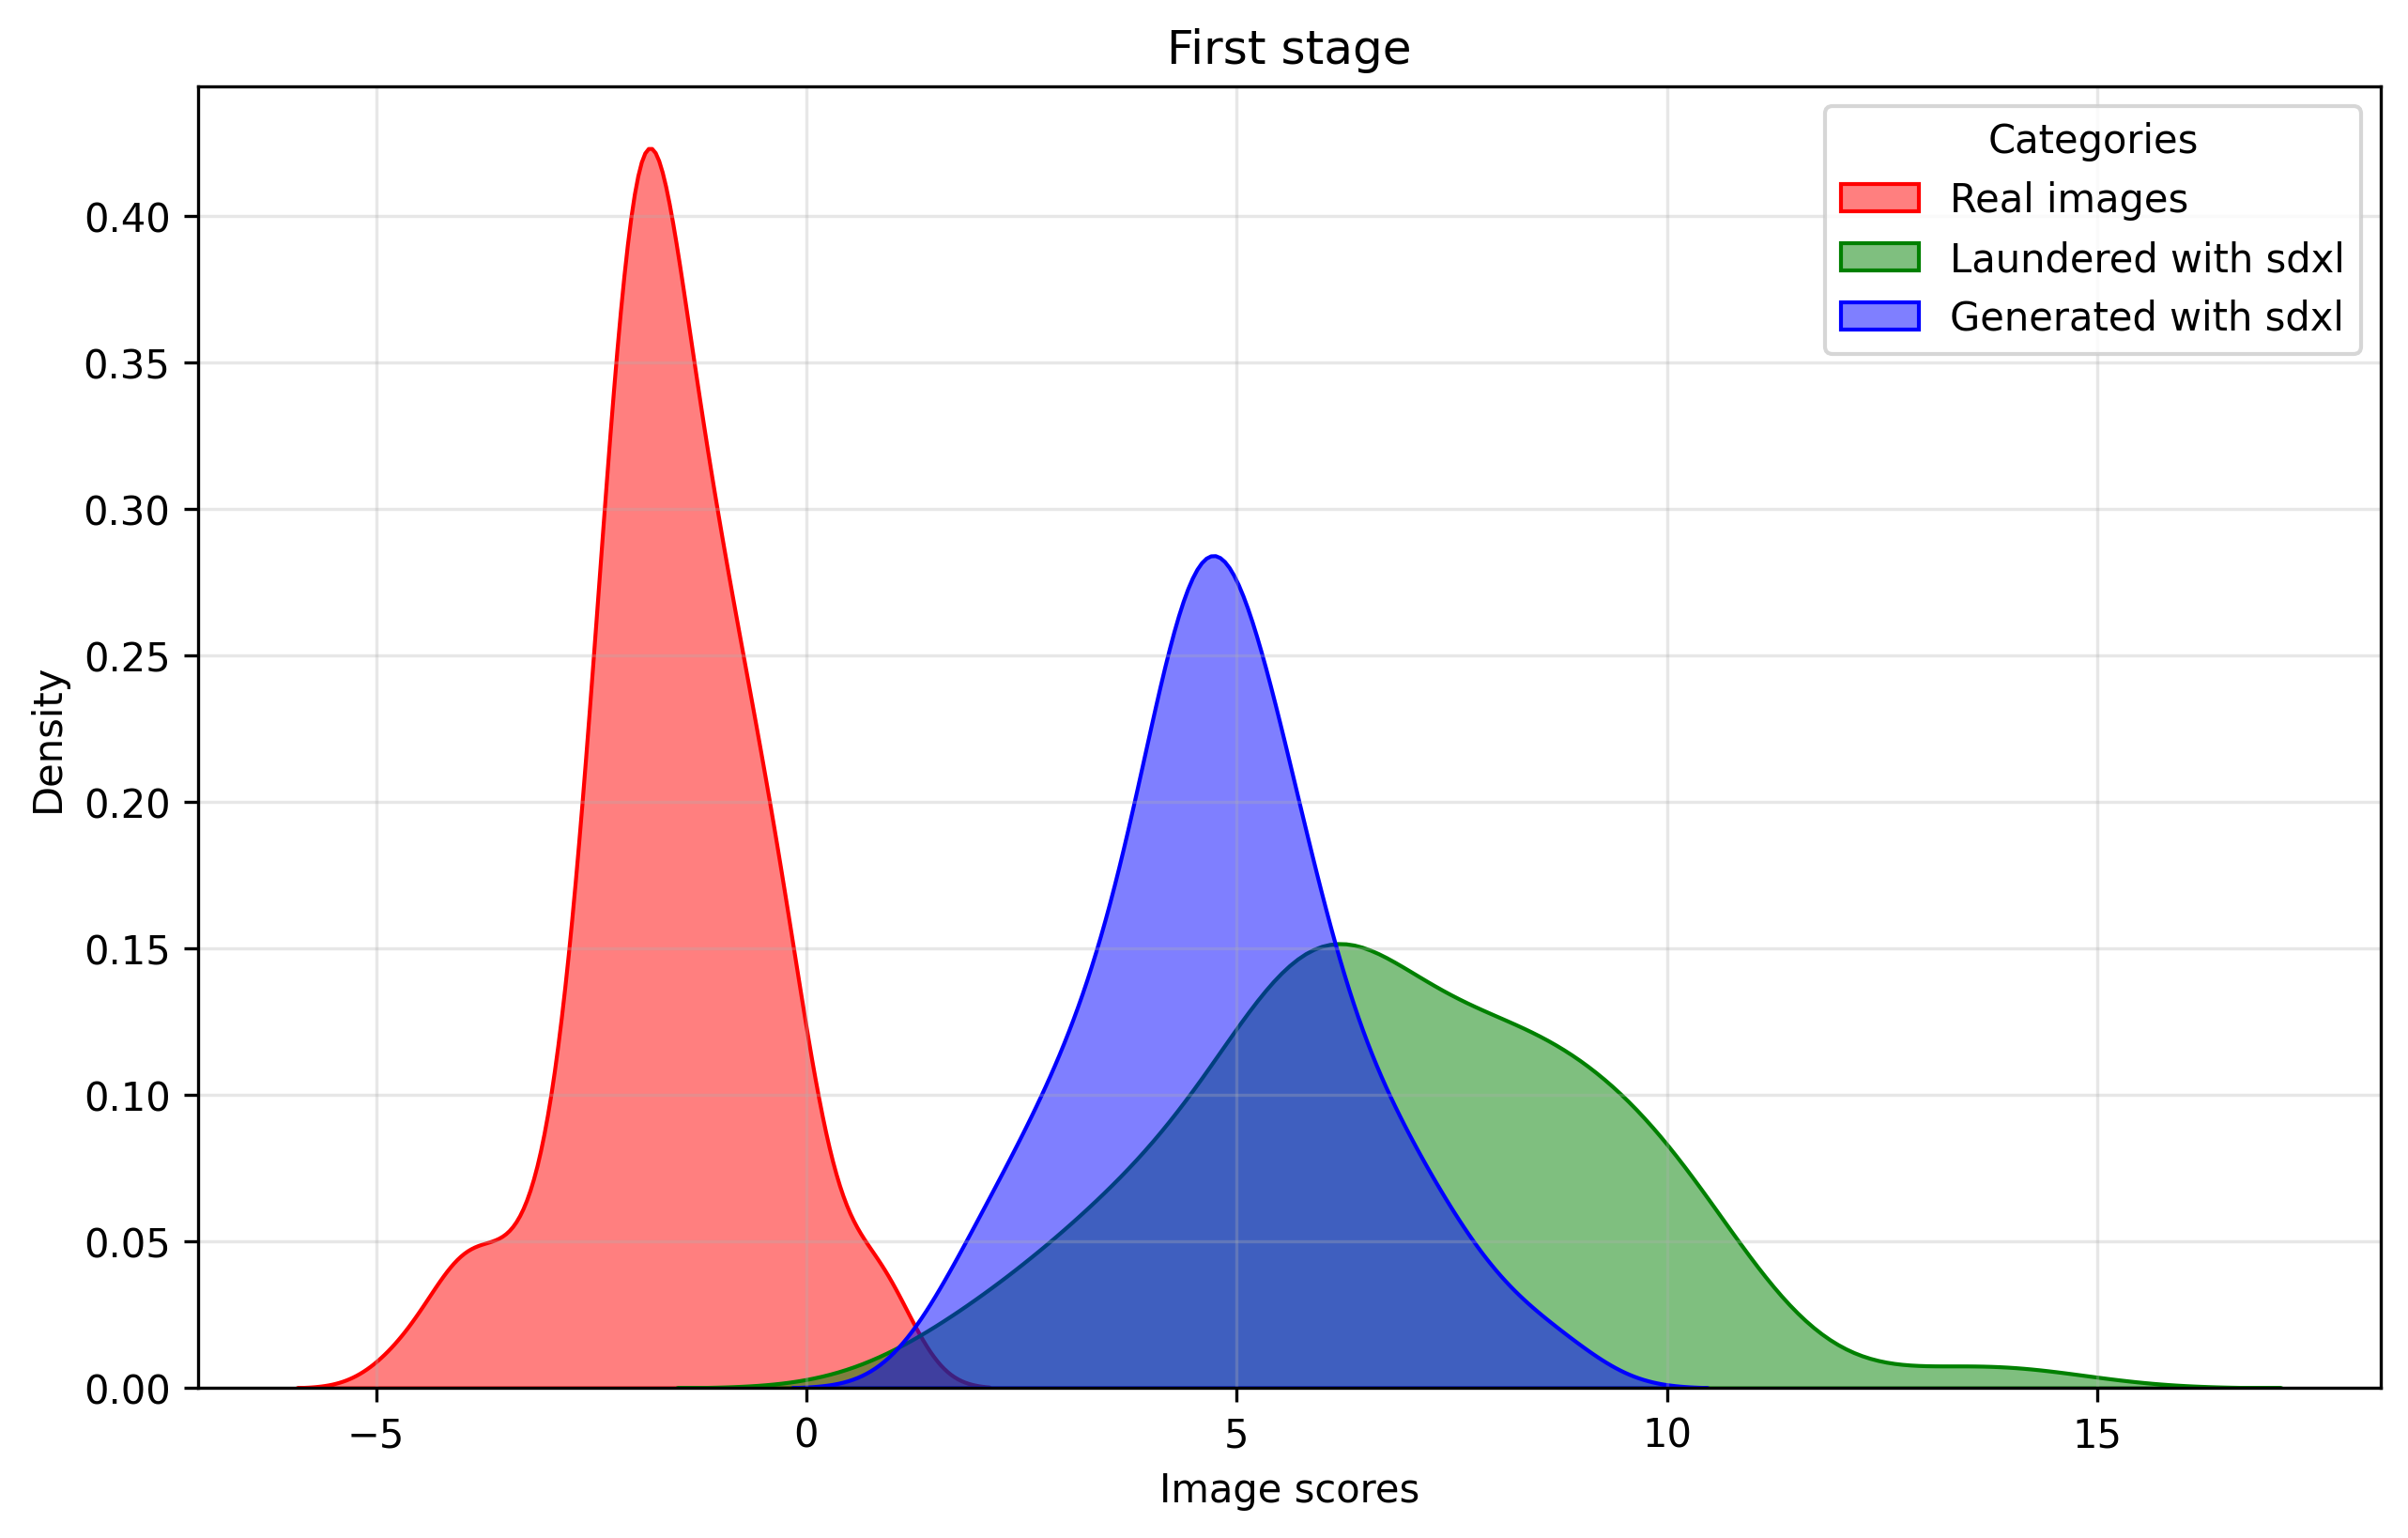
\includegraphics[width=0.8\linewidth]{Img/First_stage.png}
    %    \caption{Esempio di immagine.}
    %    \label{fig:esempio}
    %\end{figure}

\section{Detectors}
    \subsection{CLIP}
    \subsection{PIZZA}
\section{Attacks}
    \subsection{Mimicry}
    \subsection{SD Laundering}
    \subsection{White Black}
    \subsection{Adversarial Robustness}
\section{Experiment}
\section{Conclusions}

\bibliographystyle{IEEEtran} % Stile delle referenze (es. IEEE)
\bibliography{references}    % Nome del file .bib (senza estensione)

\end{document}